\section{Learning to rank}
\subsection{Introduction}
Thus far, we've looked at methods for ranking documents (e.g. cosine similarity, IDF, proximity, TF, PageRank etc..), but we've also looked at methods for classifying documents using supervised ML classifiers (e.g. Naive Bayes, Rocchio's algorithm, kNN). Now the question is: can we also \textbf{use ML} to \textbf{rank} the \textbf{documents} displayed in search results? This is the problem addressed by \textbf{learning to rank}, or \textbf{LTR}.

Some issues some years ago:

\begin{itemize}
    \item \textbf{Limited training data}: especially for real world use, it was very hard to gather test collection queries and relevance judgements that are representative of real user needs and judgements on documents returned;
    \item \textbf{Poor ML techniques};
    \item \textbf{Insufficient customization} to IR problem;
    \item \textbf{Not enough features} for ML to show value;
\end{itemize}

In this sense, traditional ranking functions in IR used a very small number of features, e.g. TF, IDF and document length.. In modern systems, especially on the Web, many features are used, e.g. log frequency of the query word in anchor text, number of images on a page, number of (out)links on a page, URL length (because if the URL is long, than probably the page is not important), BM25, URL click count etc..

\subsection{LTR}
The usual \textbf{LTR framework} is composed of:

\begin{itemize}
    \item A large training set, composed of queries and ideal document ranking. In particular, for each query, a list of $(\text{document,relevant score})$ is provided;

    \item A set of features that are used for training the ML model. Many types of features exist:

    \begin{itemize}
        \item Query-only features, i.e. query features with the same value for each document, e.g. query type, query length;
        \item Query-dependent features, i.e. document features that depend on the query, e.g. query-URL click count, BM25 etc..;
        \item Query-independent features, i.e. document features with the same value for each query, e.g. PageRank, URL length etc..
    \end{itemize}

    \item A ML model, usually a regressor, that produces a final ranked list of documents. Notice that even if the ML models are regressors that score each candidate document, the goal is to guess the overall ranking, not the specific relevance judgement labels.
\end{itemize}

, as shown in Picture \ref{ltr1}.

\begin{figure}[h!]
		\centering
        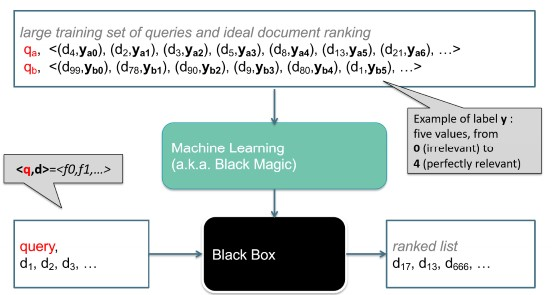
\includegraphics[scale = 1.8]{img/ltr1.jpg}
		\label{ltr1}
        \caption{LTR framework}
\end{figure}

Picture \ref{ltr2}, on the other hand, shows the pipeline of the LTR.

\begin{itemize}
    \item In the first step, the base ranker produces a first ranking of the documents, exploiting cosine similarity, BM25 etc..;
    \item Then, this ranking is provided as feature to the LTR algorithm, which in turn is used to build a top ranker (which may be composed as a cascade of rankers). Finally, this top ranker provides the user a top-$k$ documents for the given query.
\end{itemize}

\begin{figure}[h!]
		\centering
        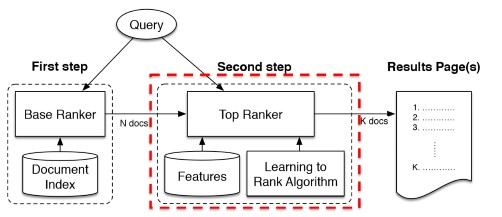
\includegraphics[scale = 1.8]{img/ltr2.jpg}
		\label{ltr2}
        \caption{LTR pipeline}
\end{figure}

Notice that budget considerations are very important for commercial Web Search Engines, so the computational cost of LTR model must be strictly accounted in the time budget available for processing queries in the incoming stream.In other words, the step of the ranking pipeline involving the LTR model must be as efficient as possible.

\subsubsection{LTR approaches}
There exist many approaches for LTR framework:

\begin{itemize}
    \item \textbf{Pointwise}: in this case \textbf{each} query-document \textbf{pair} is associated with a \textbf{score}, and the \textbf{objective} of the ML model is to \textbf{predict} such \textbf{score}. In this sense, it can be considered ad a pure \textbf{regression problem} (if the score is "continuous"), or a \textbf{multi-class classification problem} (if the score is "discrete"). Notice that this approach does not consider the position of a document into the final ranking;
    \item \textbf{Pairwise}: in this case we're given \textbf{pairwise preferences}, e.g. $d_1$ is better than $d_2$ for a query $q$, so the \textbf{objective} is to \textbf{predict} a \textbf{score} that \textbf{preserves such preferences}. In this sense, it can be considered as a \textbf{binary classification problem}. Notice that this approach does not consider the relevance of a document into the final ranking;
    \item \textbf{Listwise}: finally, in this case we're given the \textbf{ideal ranking} of results for each query, so the \textbf{objective} is to \textbf{maximize the quality of the whole resulting ranked list} by exploiting the whole list at training time. This approach is also used in recommendation systems.
\end{itemize}

In general, a modern ranking architecture should be:

\begin{itemize}
    \item \textbf{Effective}, i.e. the users should be happy of the results they receive;
    \item \textbf{Efficient}, i.e. it should have a low response time (<0.1 sec);
    \item \textbf{Easy to adapt}, i.e. it should perform a continuous crawling of the Web, exploiting users' feedback.
\end{itemize}

In this sense, the state-of-the-art is represented by \textbf{Additive Regression Trees} and \textbf{LambdaMART} models, which will be presented in the following Sections. 

We now focus on the \textit{pointwise} and \textit{pairwise} approaches.

\subsubsection{Pointwise approach}
We now discuss a first example of classification for IR. 

In this case the \textbf{training set} is composed of $(q,d,r)$ triples, where $r$ represents the relevance of each document w.r.t. a query, and it is a binary score, i.e. \textit{relevant} or \textit{not relevant}. Moreover, each document is represented by a feature vector $x = (\alpha, \omega)$, where:

\begin{itemize}
    \item $\alpha$ represents the cosine similarity;
    \item $\omega$ represents the minimum query window size, i.e. the shortest text span that includes all the query words, regardless of the order.
\end{itemize}

In this sense, the goal of the classifier is to predict the relevance $r$ of a new document-query pair. A linear score function is :

$$
\text{score}(q,d) = \text{score}(\langle \alpha,\omega \rangle) = a\alpha + b\omega
$$

, so the linear classifier has to determine the parameters $a$, $b$ and $\theta$ to decide that a document is \textit{relevant} if $\text{score}(q,d) > \theta$, and \textit{not relevant} if $\text{score}(q,d) \leq \theta$. This methodology is usually referred as \textbf{pointwise ranking}. A visual representation of such classifier is provided in Picture \ref{class rank}.

\begin{figure}[h!]
		\centering
        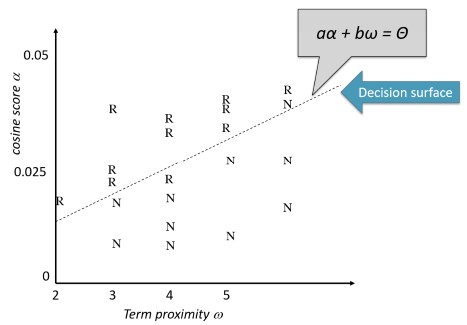
\includegraphics[scale = 1.8]{img/classification ranking.jpg}
		\label{class rank}
        \caption{Linear classifier}
\end{figure}

\subsection{BM25 and BM25F}
\textbf{BM25} is a \textit{probabilistic} ranking function, \textit{state-of-the-art} method that exploits term independence assumption to \textbf{approximate} the \textbf{probability} of a \textbf{document} of being \textbf{relevant}. The BM25 score is define as:

$$
\text{score}_{\text{BM25}}(q,d) = \sum_{q_t \in q} TF_{\text{BM25}}(q_t,d) \cdot IDF(q_t)
$$

, where:

\begin{itemize}
    \item $IDF(q_t) = \log (\frac{|D|}{DF(q_t)})$. Notice that since $DF(q_t)$ is in the denominator, the more documents contain a term, i.e. the more frequent a term is, the less contribution the term given to the score;
    \item $TF_{\text{BM25}}(q_t,d) = \frac{TF(q_t,d)}{k + 1 - b + b \frac{l_d}{L}}$, where $l$ represents the length of document $d$, and $L$ the average document length in the collection. Notice that the parameter $b$ determines the importance of $l_d$ w.r.t. $L$. 
    
    In general, if $l_d = L$, then $TF_{\text{BM25}}(q_t,d) = TF(q_t, d)$; if $l_d >> L$, for example $l_d = 2L$, then $TF_{\text{BM25}}(q_t,d) = \frac{TF(q_t,d)}{1+b}$, so we penalize more the contribution of the term frequency. In other words, $\frac{l_d}{L}$ penalizes or awards the term frequency following the schema of Picture \ref{bm25 1}.

    \begin{figure}[h!]
		\centering
        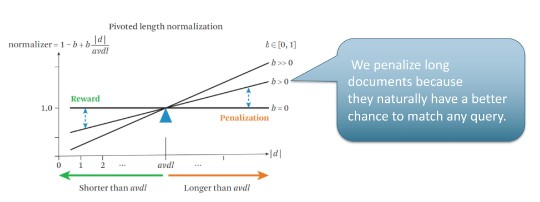
\includegraphics[scale = 1.8]{img/bm251.jpg}
		\label{bm25 1}
        \caption{Parameter $b$}
    \end{figure}
\end{itemize}

BM25 can be extended to handle \textit{structure documents}, i.e. multi-field documents, where a field could be the title, the abstract, the body etc.. The extended function is called \textbf{BM25F}, and it is define as:

$$
\text{score}_{\text{BM25F}}(q,d) = \sum_{q_t \in q} TF_{\text{BM25F}}(q_t,d) \cdot IDF(q_t)
$$

, where 

$$
TF_{\text{BM25F}} = \sum_{s} \frac{w_s \cdot TF(q_t, s)}{1 - b_s + b_s \frac{l_s}{L_s}}
$$

, where:

\begin{itemize}
    \item $s$ represents a field;
    \item $w_s$ is the weight of field $s$ (of document $d$);
    \item $l_s$ is the length of field $s$ (of document $d$);
    \item $b_s$ determines the importance of $l_s$;
    \item $L_s$ is the average length of field $s$ in the collection.
\end{itemize}

We notice that while BM25 has two parameters, $b$ and $k$, BM25F has $2S + 1$ free parameters, where $S$ is the total number of fields: indeed, we have $b_s$ and $w_s$ for each of the $S$ fields, plus the parameter $k$. Thus, in order to find the best parameters of BM25(F), we can fit it into a LTR framework.

\subsection{LTR for BM25(F)}
In general, the three main ingredients for exploiting ML in our system are:

\begin{itemize}
    \item An \textbf{evaluation function}, i.e. a method for evaluating our results;
    \item The \textbf{ML algorithm}, and in particular the hypothesis space (linear combination, mixture models, etc..) and the optimization strategy (greedy, bounded approximation etc..);
    \item The \textbf{data}.
\end{itemize}

\subsubsection{Using NDCG}

In the case of BM25(F), we consider:

\begin{itemize}
    \item The \textit{NDCG@k} as evaluation function;
    \item As ML model, we must search over all the possible BM25(F) functions, using a gradient descent strategy over NDCG@k;
    \item The data are composed of a set of query/results, where each query has a set of candidate results, each of which was manually annotated with a relevance label (e.g. from 0 to 4).
\end{itemize}

In particular, given a query $q$ and a set of documents $D = \{ d_1, d_2, .. \}$, we want to learn a model $h$ that allows to score and then rank the documents in $D$ according to their relevance. In this sense, the results will be $\text{sort}\{ h(d_1), h(d_2), .. \}$, where the model $h$ is BM25F with a proper parameter set $\theta$.

However, if we want to apply the gradient descent strategy, we would need to compute the gradient of the sort function w.r.t. $\theta$, but sort is not a continuous and differentiable function, so we cannot apply this strategy.

The first solution to this problem is to optimize by \textbf{line search}, i.e. from a point in the parameter space, we perform a line search along each individual parameter co-ordinate axis, i.e. we try many values for each parameters, while the other are kept fixed. In our case, this means that NDCG is computed for each of the $N$ sample points along the line, and the location of the best NDCG is recorded.

\subsubsection{Pairwise approach}
However, since NDCG cannot be directly optimized, we can change completely the optimization strategy by considering \textbf{pairwise} ordering. In this case we're given a collection $R$ of document pairs $(d_i,d_j)$, and for each pair we know that $d_i$ is more relevant that $d_j$: our goal is to find the \textbf{best ranking function} $r^*$ s.t. for each pair $(d_i, d_j) \in R$, $r^*(d_i) < r^*(d_j)$, where smaller ranks are better. In other words, the goal is to find the ranking function s.t. the smallest number of such constraints is violated. We now consider the \textbf{RankNet} approach.

Let the \textbf{training set} be \textbf{result pairs} $(d_1,d_2)$ where $d_1$ is better than $d_2$ (we also say that the \textit{true probability} that $d_1$ is better than $d_2$ is $T_{12} = 1$). Let $h(d)$ be the \textbf{score} of document $d$ computed by the learned model: obviously, the higher the score, the better, and the document ranking is obtained by sorting the documents in decreasing order of $h(d)$. We then define the \textbf{score difference} $Y = h(d_1) - h(d_2)$: if $Y > 0$, then the documents are ranked correctly. We now \textbf{map} $Y$ to the probability $P_{12}$ that $d_1$ is better than $d_2$ with a \textbf{sigmoid function}:

$$
P_{12} = \frac{1}{ 1+ e^{-Y}}
$$

We now measure the \textbf{error of the model} using the \textbf{cross entropy} between $P_{12}$ and $T_{12}$:

$$
C_{12} = -T_{12} \log P_{12} - (1 - T_{12}) \log (1-P_{12})
$$

Notice that:

\begin{itemize}
    \item The \textbf{cross entropy} is used to define a \textbf{loss function} in ML and optimization;
    \item Thus, in this case, it aims to \textbf{minimize} the number of inversions in ranking.
\end{itemize}

However, since we take the pair ordering of the training set as certain , then $T_{12} = 1$, so the loss function reduces to:

$$
C_{12} = \log (1 + e^{-Y})
$$

In this sense, the overall RankNet loss is defined as:

$$
C = \sum_{d_i,d_j} C_{ij} = \sum_{d_i,d_j} \log (1 + e^{-Y})
$$

We have that $C$ is \textbf{minimum} if all pairs are ranked in the proper order, therefore my minimizing $C$ we aim at \textbf{improving NDCG}. Notice that now $C$ is a continuous function, so we can compute its \textbf{gradient} and directly apply \textbf{steepest descent}.

Thus, in this case the LTR framework is composed of:

\begin{itemize}
    \item A proxy of the \textit{NDCG@k} evaluation function, the \textit{RankNet cost};
    \item As a ML model, we still must search over all the possible BM25(F) functions, using a gradient descent strategy over RankNet cost;
    \item The data the same as before.
\end{itemize}

The results showed that this alternative formulation using the RankNet cost is a good proxy for NDCG optimization. However, the \textbf{pairwise approach} has some \textbf{disadvantages}. We know that its goal is to maximize the number of correctly classified pairs, but in general the number of document pairs violations might not be a good indicator, since errors that occurs at the bottom of the ranking are not the same as errors at the top of the ranking.

\subsection{LambdaMART}

\subsubsection{Decision Tree and Regression Tree}
We start our discussion by introducing the concept of \textbf{decision tree}. A decision tree is a tree-like structure in which each \textbf{internal node} denotes a \textbf{test} over an attribute/feature, and each \textbf{leaf node} is associated with a \textbf{class label}, in case of a classification task, or a \textbf{predicted value}, in case of a regression task. A visual representation of a decision tree is provided in Picture \ref{dt}.

\begin{figure}[h!]
		\centering
        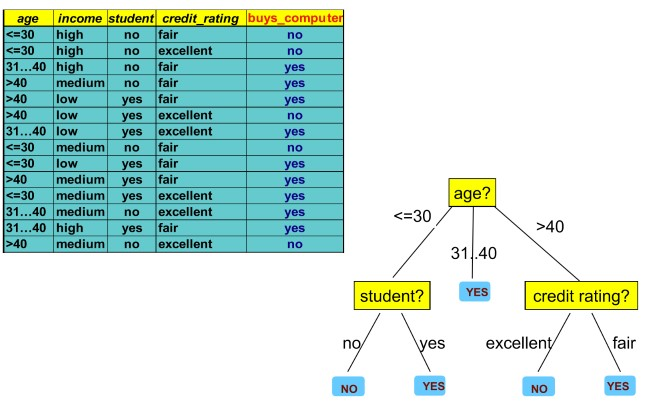
\includegraphics[scale = 1.8]{img/decision tree.jpg}
		\label{dt}
        \caption{Example of decision tree}
\end{figure}

Then, the decision tree is used to label a new data instance on the basis of its structure: it runs several tests on the data instance attributes and it traverses the tree according to the tests results. The label associated to the leaf represents the prediction of the decision tree.

In case of a regression task, a \textbf{regression tree} is used: a regression tree is a tree in which each \textbf{internal node} is a predicate on some feature, and a \textbf{leaf} is a prediction. Given a set of features $X = \{ X_1, X_2, .. \}$, the goal is to find the tree that best predicts $Y$ on the training data. An example is provided in Picture \ref{rt}.

\begin{figure}[h!]
		\centering
        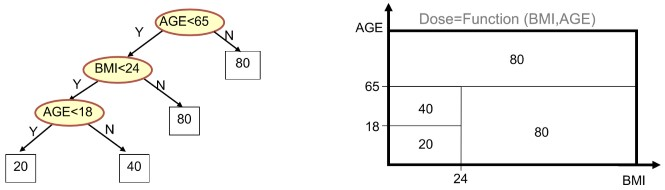
\includegraphics[scale = 1.8]{img/regression tree.jpg}
		\label{rt}
        \caption{Example of regression tree}
\end{figure}

Notice that in both the decision tree and the regression tree, each node induces a partitioning/splitting of the data.

Now the question is: how do we build a decision/regression tree? We must recursively decide the best feature for which performing a split of the dataset. The \textbf{best split} can be decided using a \textbf{greedy strategy}: for each possible candidate, i.e. for each \textbf{splitting criterion}, compute the prediction for the left and right child, where the prediction is given by the average of the target variable on the corresponding instances. Then, the \textbf{goodness of the split} is computed as an error reduction (usually MSE), and the split with best \textbf{error reduction} is chosen. Then, the data are splitted according to the chosen split criterion, and the operations are repeated recursively on the sub-trees.

The \textbf{advantage} of a decision/regression tree is that it is very \textbf{explainable}, in the sense that a single prediction/classification can be easily analyzed by traversing the tree, but a \textbf{disadvantage} is that it is not very powerful for some tasks, and it is also prone to \textbf{overfitting}.

\subsubsection{Ensemble of trees}
In order to overcome the problems of a single decision/regression tree, an \textbf{ensemble method} can be exploited. An ensemble is a combination of trees that is able to combine their predictive power by reducing the overfitting problem. A famous technique for building an ensemble is \textbf{bagging}, which essentially performs a bootstrap operation and an aggregation.

An example of ensemble of trees is a \textbf{random forest}, which is a collection of randomly created decision trees, in which each test node in a decision tree works on a random subset of the features, and the final forest then combines the output of individual decision trees to generate the final output, e.g. by averaging the trees' leave values. A representation is provided in Picture \ref{rf}.

\begin{figure}[h!]
		\centering
        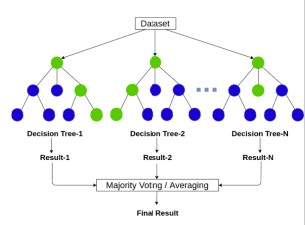
\includegraphics[scale = 1.8]{img/ensemble of trees.jpg}
		\label{rf}
        \caption{Example of Random Forest}
\end{figure}

\subsubsection{MART}
\textbf{MART} (Multiple Additive Regression Trees) is an \textbf{ensemble of trees} adopting \textbf{gradient boosting}. A gradient-boosted tree model is built on a stage-wise fashion as in other boosting methods:

\begin{itemize}
    \item The model iteratively learns a weak learner, e.g. a shallow decision tree;
    \item Then, it adds this weak learner to the final strong classifier, i.e. to the ensemble;
    \item The next weak learner will focus more on mis-classified data items.
\end{itemize}

In this sense, MART is also known as \textbf{Gradient Boosting Regression Tree} (\textbf{GBRT}).

From a mathematical point of view, given a ground truth $D = \{ (x_1, y_1), .., (x_{|D|}, y_{|D|}) \}$, where $x \in \mathbb{R}^{|F|}$ (in our case $x = (\text{query}, \text{doc})$ and $y_i = \text{score}$), GBRT learns incrementally an ensemble of $m$ trees predicting the various $y_i$:

$$
F_m(x) = F_{m-1}(x) + v \cdot h_m(x)
$$
, where:

\begin{itemize}
    \item $F_{m-1}(x)$ represents the summation of all the outputs of the trees in the ensemble so far;
    \item $h_m(x)$ represents the output of the current tree;
    \item $v$ is a \textbf{shrinkage factor} or learning rate, which act as a regularization factor by shrinking the minimization step along the steepest descent direction.
\end{itemize}

Notice that $h_m(x)$ is sufficiently easy to be learnt, since it represents the output of a relatively shallow tree, and its goal is to reduce the error/cost function of $F_{m-1}(x)$ learned so far. When the method starts, $h_0$ represents the initial guess, e.g. the average of the various $y_i$.

The function $F(x)$ learned by GBRT minimizes a loss function that is averaged over all $x_i$, usually the mean squared error:

$$
L(y_i,F(x_i)) = \frac{1}{2} (y_i - F(x_i))^2
$$

Then, since we exploit the steepest descent method, we must compute the negative gradient:

$$
- g_m(x_i) = \frac{\partial L(y_i, F(x_i))}{\partial F(x_i)}|_{F(x) = F_{m-1}(x)} = y_i - F_{m-1}(x_i)
$$

Intuitively, to improve our prediction for $x_i$, we have to fit a new regression tree $h_m$ whose output is $y_i - F_{m-1}(x_i)$, which are called \textbf{residuals}.

Now, the question is: can we optimize NDCG rather than MSE? No, since we cannot compute the derivative function of NDCG. However, we showed that RankNet cost represents a good proxy for that measure: for this reason, we now introduce Lambda-Rank.

\subsubsection{Lambda-Rank}
\textbf{Lambda-Rank} is a GBRT that optimizes directly the derivable \textbf{RankNet pairwise loss}, i.e. it provides a new way for computing the residuals. In this case, the \textbf{gradients} $\lambda$ of the cost w.r.t. the model score can be seen as \textbf{little arrows} attached to each document in the ranked list, indicating the direction we would like those documents to move to reduce the number of \textbf{pairwise violations}. In particular, we have that:

$$
\lambda_{ij} = \frac{\partial C(s_i - s_j)}{\partial s_i} = \frac{1}{1 + e^{s_i - s_j}}
$$
, where $s_i$ and $s_j$ are the scores produced by the model that we're training, i.e. $s_i = F_{m-1}(x_i)$ and $s_j = F_{m-1}(x_j)$.

Then, we assign a gradient $\lambda_i$ to each document $d_i$ for a given query $q$:

$$
\lambda_i^q = \sum_{j:(i,j) \in I^q} \lambda_{ij}^q - \sum_{j:(j,i) \in I^q} \lambda_{ji}^q
$$

, where $I^q = \{ (i,j) : y_i^q > y_j^q \}$, i.e. the set of all the document pairs $(i,j)$ ranked according to the relevance judgements $y_i$ and $y_j$ for a given query $q$. 

In this sense, if we think of each $\lambda$ as a force applied to documents, the first sum accounts for all the forces coming from less relevant documents, which therefore pushes $d_i$ up in the ranking; on the other hand, the second sum, finally subtracted, accounts for all the forces coming from more relevant documents, which therefore pushes $d_i$ down in the ranking. A visual representation of this behaviour is provided in Picture \ref{forces}.

\begin{figure}[h!]
		\centering
        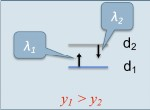
\includegraphics[scale = 2.5]{img/forces.jpg}
		\label{forces}
        \caption{$\lambda_i$ as a force}
\end{figure}

As we can see, in this case $y_1 > y_2$, i.e. the relevance judgement of $y_1$ is greater than the relevance judgement of $y_2$, but the ranking is different. For this reason, $\lambda_1$ forces $d_1$ up in the ranking, while $\lambda_2$ forces $d_2$ down in the ranking.

In general, Lambda-Rank is a good model, since it tries to minimize the pairwise violations, but still is not able to directly optimize NDCG. For this reason, we now discuss about Lambda-MART.

\subsubsection{Lambda-MART}
\textbf{Lambda-MART} uses an approximation of NDCG gradient. In particular, for each training instance $x_i$, Lambda-MART estimates the \textbf{benefit of increasing or decreasing} the currently predicted score $F_{m-1}(x_i)$ in terms of NDCG.

The new $\lambda$-gradient $\lambda_i$ is computed as a before, but we multiply each $\lambda_{ij}$ by $|\Delta NDCG_{ij}|$: after sorting by score the documents for each query $q$, for each pair $(i,j)$ where the $i$-th document is more relevant the the $j$-th, i.e. $(i,j) \in I^q$, we compute $|\Delta NDCG_{ij}|$. Indeed, $|\Delta NDCG_{ij}|$ is the change in terms of NDCG given by swapping the rank positions of $d_i$ and $d_j$, while leaving the other documents untouched.

In this sense, the new residuals are:

$$
\lambda_{ij} = \frac{1}{1 + e^{s_i - s_j}} \cdot |\Delta NDCG|
$$

Picture \ref{lambda mart} provides a comparison between plain RankNet $\lambda$'s (black arrows) and Lambda-MART one's (red arrows); notice that in the Picture, the blue indicates a relevant document. 

\begin{figure}[h!]
		\centering
        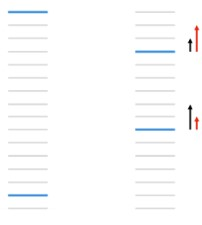
\includegraphics[scale = 2.5]{img/lambda mart.jpg}
		\label{lambda mart}
        \caption{Comparison between plain RankNet $\lambda$'s and Lambda-MART one's}
\end{figure}

In the left we see a ranking that is very good in terms of NDCG, despite having a higher number of pairwise violations (13), while in the right we notice how RankNet $\lambda$'s try to increase the score of the second relevant document more than Lambda-MART, since its goal is to minimize the number of pairwise violations. Moreover, we notice how the first relevant document is heavily pushed up by Lambda-MART, since optimizing NDCG, its goal is to have relevant documents in the first positions.

As a resume, in Lambda-MART framework is composed of:

\begin{itemize}
    \item The \textit{NDCG@k} as evaluation function;
    \item As ML model, must search over a sum of regression trees, where each tree is fitted w.r.t. new residuals, and injecting the evaluation function into the gradient of RankNet's cost;
    \item The data are the same as before.
\end{itemize}